\documentclass[man,floatsintext]{apa6}
\usepackage{lmodern}
\usepackage{amssymb,amsmath}
\usepackage{ifxetex,ifluatex}
\usepackage{fixltx2e} % provides \textsubscript
\ifnum 0\ifxetex 1\fi\ifluatex 1\fi=0 % if pdftex
  \usepackage[T1]{fontenc}
  \usepackage[utf8]{inputenc}
\else % if luatex or xelatex
  \ifxetex
    \usepackage{mathspec}
  \else
    \usepackage{fontspec}
  \fi
  \defaultfontfeatures{Ligatures=TeX,Scale=MatchLowercase}
\fi
% use upquote if available, for straight quotes in verbatim environments
\IfFileExists{upquote.sty}{\usepackage{upquote}}{}
% use microtype if available
\IfFileExists{microtype.sty}{%
\usepackage{microtype}
\UseMicrotypeSet[protrusion]{basicmath} % disable protrusion for tt fonts
}{}
\usepackage{hyperref}
\PassOptionsToPackage{usenames,dvipsnames}{color} % color is loaded by hyperref
\hypersetup{unicode=true,
            pdftitle={Sociotechnical energy imaginaries of non-users of ECO-innovations: identification and perceptions of residential households not adopting solar energy},
            pdfauthor={Marco Bunt},
            pdfkeywords={future imaginaries, Sustainability, ECO-innovation, diffusion of
innovation,non-adopters},
            colorlinks=true,
            linkcolor=blue,
            citecolor=Blue,
            urlcolor=Blue,
            breaklinks=true}
\urlstyle{same}  % don't use monospace font for urls
\usepackage{graphicx,grffile}
\makeatletter
\def\maxwidth{\ifdim\Gin@nat@width>\linewidth\linewidth\else\Gin@nat@width\fi}
\def\maxheight{\ifdim\Gin@nat@height>\textheight\textheight\else\Gin@nat@height\fi}
\makeatother
% Scale images if necessary, so that they will not overflow the page
% margins by default, and it is still possible to overwrite the defaults
% using explicit options in \includegraphics[width, height, ...]{}
\setkeys{Gin}{width=\maxwidth,height=\maxheight,keepaspectratio}
\IfFileExists{parskip.sty}{%
\usepackage{parskip}
}{% else
\setlength{\parindent}{0pt}
\setlength{\parskip}{6pt plus 2pt minus 1pt}
}
\setlength{\emergencystretch}{3em}  % prevent overfull lines
\providecommand{\tightlist}{%
  \setlength{\itemsep}{0pt}\setlength{\parskip}{0pt}}
\setcounter{secnumdepth}{0}
% Redefines (sub)paragraphs to behave more like sections
\ifx\paragraph\undefined\else
\let\oldparagraph\paragraph
\renewcommand{\paragraph}[1]{\oldparagraph{#1}\mbox{}}
\fi
\ifx\subparagraph\undefined\else
\let\oldsubparagraph\subparagraph
\renewcommand{\subparagraph}[1]{\oldsubparagraph{#1}\mbox{}}
\fi

%%% Use protect on footnotes to avoid problems with footnotes in titles
\let\rmarkdownfootnote\footnote%
\def\footnote{\protect\rmarkdownfootnote}


  \title{Sociotechnical energy imaginaries of non-users of ECO-innovations:
identification and perceptions of residential households not adopting
solar energy}
    \author{Marco Bunt\textsuperscript{1,2}}
    \date{}
  
\shorttitle{Sociotechnical energy imaginaries of non-users}
\affiliation{
\vspace{0.5cm}
\textsuperscript{1} Erasmus school of social and behavioural sciences\\\textsuperscript{2} Stedin netbeheer}
\keywords{future imaginaries, Sustainability, ECO-innovation,  diffusion of innovation,non-adopters\newline\indent Word count: 2900}
\usepackage{csquotes}
\usepackage{upgreek}
\captionsetup{font=singlespacing,justification=justified}

\usepackage{longtable}
\usepackage{lscape}
\usepackage{multirow}
\usepackage{tabularx}
\usepackage[flushleft]{threeparttable}
\usepackage{threeparttablex}

\newenvironment{lltable}{\begin{landscape}\begin{center}\begin{ThreePartTable}}{\end{ThreePartTable}\end{center}\end{landscape}}

\makeatletter
\newcommand\LastLTentrywidth{1em}
\newlength\longtablewidth
\setlength{\longtablewidth}{1in}
\newcommand{\getlongtablewidth}{\begingroup \ifcsname LT@\roman{LT@tables}\endcsname \global\longtablewidth=0pt \renewcommand{\LT@entry}[2]{\global\advance\longtablewidth by ##2\relax\gdef\LastLTentrywidth{##2}}\@nameuse{LT@\roman{LT@tables}} \fi \endgroup}


\usepackage[titles]{tocloft}
\cftpagenumbersoff{figure}
\renewcommand{\cftfigpresnum}{\itshape\figurename\enspace}
\renewcommand{\cftfigaftersnum}{.\space}
\setlength{\cftfigindent}{0pt}
\setlength{\cftafterloftitleskip}{0pt}
\settowidth{\cftfignumwidth}{Figure 10.\qquad}
\cftpagenumbersoff{table}
\renewcommand{\cfttabpresnum}{\itshape\tablename\enspace}
\renewcommand{\cfttabaftersnum}{.\space}
\setlength{\cfttabindent}{0pt}
\setlength{\cftafterloftitleskip}{0pt}
\settowidth{\cfttabnumwidth}{Table 10.\qquad}

\authornote{This article is the graduation thesis om Marco
Bunt for the study social science on the Erasmus school of social and
behavioral sciences, in collaboration with Stedin.

Correspondence concerning this article should be addressed to Marco
Bunt, Stedin, Blaak 8, 3011 TA Rotterdam. E-mail:
\href{mailto:marco.bunt@Stedin.net}{\nolinkurl{marco.bunt@Stedin.net}}}

\abstract{
Yet to be written


}

\begin{document}
\maketitle

\section{Introduction}\label{introduction}

In the process of modernization, unsustainability is produced as a
side-effect of economic and technological development (IPCC, 2014). The
unsustainability becomes visible in the over-consumption of natural
resources, loss of biodiversity and climate change problems. To overcome
these problems, climate change urges national and local governments to
make policies to enable energy transition from fossil energy sources
that are free from emitting carbon in the atmosphere. The Dutch
government aims to reduce the emission of carbon by 50\% or more before
2030. One of the challenges in this vision is the transformation of more
than 7 million houses, mostly moderately insulated and almost all heated
by natural gas, to well-insulated houses, headed with energy from a
sustainable source and in which clean electricity is used (EZK, 2019, p.
21). This goal means an extensive and expansive transformation of the
Dutch society where everyone has to participate. The technology used for
achieving this goal is mainly decentralized power generation through
photovoltaic solar panels (PV), windmills and heat pumps (HP).
Fossil-based transport shall be replaced by electric vehicles (EV),
either with batteries or hydrogen (EZK, 2019). Technologies like these
that enable a more sustainable way of living are addressed as called
\enquote{ECO-innovations} (James, 1997) in this article, as described in
the theoretical framework of this article.

These new technologies are more likely to be adopted by people that have
more (Rogers, 1983), and thereby improve their position in relative
comparison to the people that are unable to adopt(Gladwell, 2013;
Merton, 1968). Thereby people that can innovate can sustain their
lifestyle as consumers while lowering their environmental impact with
the help of government subsidies, while people that are not adopting the
new technology can only create a sustainable lifestyle by consuming less
(Jhagroe \& Loorbach, 2015). In this way, Jhagroe (2016) argues that the
transitions increase the already existing gap between rich and poor. A
large amount of research is devoted to identifying innovators in general
(Bogers, Afuah, \& Bastian, 2010) and innovators of sustainable
technology such as PV (Vasseur \& Kemp, 2015). However, there is not
much theory (that we know of) about the people who are not transitioning
themselves to sustainable forms of energy. Therefore academic research
on this topic is needed. Late adopters of an innovation are most likely
to be individually blamed for not adopting an innovation or for being
much later in adopting than the other members of their system, while
careful analysis can show that an innovation maybe is not appropriate
for this group (Rogers, 1983). Therefore it is important to study the
people that are not adopting sustainable innovations in the present-day
energy transition, to prevent stigmatization for this group. In
understanding why the group is not adopting this, this article gains
social relevance. This article studies the people that are not adopting
ECO-innovations by conducting a mixed-method inquiry, including a
quantitative part to identify the non-adopters, and a qualitative part
to understand why they are not adopting. The former part is done via a
multivariate regression analysis on the spatial diffusion of PV to find
parameters predicting people not adopting. The latter part is done by
conducting semi-structured interviews with people from the identified
groups.

\section{Problem statement}\label{problem-statement}

The (potential) disruptive effect that the energy transition has on the
Dutch society creates a needs to precisely identify and understand the
precarious publics that are - by not adopting -- targeted by the process
of innovating to a carbon-free society. According to Rogers, late
adopters are stereotypically perceived as being traditional, uneducated,
resistant to change, low economic resources, and that may become a
self-fulfilling prophecy (Merton, 1995; Rogers, 1983, p. 107). However,
the choice to adopt is also not only a matter of economic resources. A
division of adopters vs.~not adopters of new sustainable energy
technology's merely on the availability of recourses neglects other
motivations (Wyatt, 2003). This reasoning ignores that technological
innovation is always an interplay between material and social landscapes
(Jasanoff \& Kim, 2015). Due to both the risk and uncertainty of climate
change, people use different discourses to depict the future (Cook,
2018). This process, which Jasanoff calls \enquote{co-production,} is
about how knowledge about the world is inseparable from how we choose to
live in it (2004). The adoption of innovation is, in that manner,
influenced by individual and public visions of the desirable future in
terms of social practices, identities, norms, and instruments. These
imaginaries are diverse, and thereby both innovators and non-innovators
can be divided into numerous publics for innovation discourse. Thus the
economic resources of adopters are maybe not a motivator for innovation
increasing the possibility of adoption on a continues scale as suggested
by research (Bernards, Morren, \& Slootweg, 2018), but more as an
enabler with a threshold from where the investment becomes possible.
Sociotechnical imaginaries shape the future of the transition to a
sustainable future, understanding this imaginaries for the non-adopters
is key in understanding why this group is not innovating.

\begin{figure}

{\centering 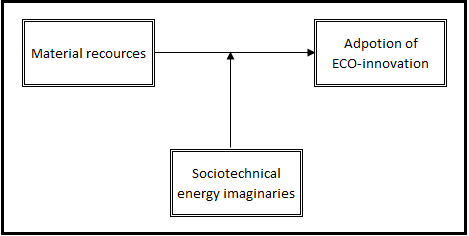
\includegraphics[width=0.75\linewidth]{C:/Users/602956/Desktop/Studie/Thesis/Sociology thesis/fig/ConceptueelModel} 

}

\caption{Conceptual model adaptation of sustainable technology}\label{fig:Conspt}
\end{figure}

The real decision making for the investment in ECO-innovation is an
interplay between the natural resources and the social world of the
adopter, the effects this interplay has on the possibility of a
household (not) to invest in sustainable innovations will be
investigated in this article. Only the investigation of the interplay
between these concepts will create an understanding of why household are
not adopting new technology. This understanding makes possible public
issues in the transition to sustainable energy visible and can thereby
help in creating a more inclusive framework for transitions. The
conceptual model is shown in figure \ref{fig:Conspt}. Built from the
findings from Rogers that laggards non-adopters are not just opposing to
change, but can experience real boundaries in adopting innovation
(Rogers, 1983), the research question in this article is the following:

\emph{What is the role of sociotechnical energy imaginaries, like
climate apocalypse or sustainable future, in the adoption of
ECO-innovation by residential households in the Dutch society?}

This question is investigated in two parts. The first part of the
research in this article is about identifying different social groups in
the adoption of innovation based on natural resources, by an empirical
study of the distribution of ECO-innovations in the Dutch landscape
(James, 1997). By investigating the material factors, such as annual
income, house ownership and characteristic of the house itself. By
studying these factors, we create more insight into the factors that
enable a household to adopt new technology. The social systems that are
identified as not adopting ECO-innovation are further investigated in
the second part of the article. This second part is an exploration of
the normative framework of the social network of a household. This part
is done by conducting extensive interviews amongst identified groups.

\section{Theoretical framework}\label{theoretical-framework}

To investigate the sociotechnical imaginaries of the people that are not
adopting an innovation, this article explores the normative framework of
people from this group concerning sustainability. This chapter explains
what we mean when we talk about imaginaries, the diffusion of
ECO-innovation and social influence.

\subsection{Sociotechnical energy
imaginaries}\label{sociotechnical-energy-imaginaries}

Imaginaries describe the way people imagine their social surroundings
and is made visible in images, stories, and legends, necessary for a
common understanding of practices and a widely shared sense of
legitimacy of things like borders and nationalities (Taylor, 2004).
These shared understandings are embedded in social practices that shape
the future through the development of, e.g., norms, policies, and
technology. Before shooting into space, it is first the imagination
dreaming about it (Jasanoff \& Kim, 2009). Methods to investigate the
role of imaginaries in the production of technology are conceptualized
in the interpretive framework of CO-production by Jasanoff and Kim
(2015) and argues that the interpretation of knowledge depends on the
interest of society. Though they can originate in the visions of single
individuals, sociotechnical imaginaries are collectively held by making
the image public and brings together the normativity of the imagination
with the materiality of networks in the production on technological
{[}energy{]} projects. Adaptation of new technology is thereby not
merely a matter of ability, but also a matter of vision. In the
adaptation of PV, the public image is complicated by the depiction of
the climate. Levy and Spices (2013) convincingly derive differed
imaginaries from observation and analysis of the various framings of the
climate actors and the media on sustainability. These four core
imaginaries they identify are the 1) \enquote{fossil fuels forever}:
this (obsolete) popular imaginary viewed abundant cheap fossil fuel as
the prime motor behind competitive industrialization. 2) the
\enquote{climate apocalypse} imaginary paints an alarming picture of the
coming decades, visible in movies like \enquote{day after tomorrow}
(\emph{The day after tomorrow}, 2004). The article of Cook (2018) shows
that people that hold this imaginary see change as inevitable and
attempts to avoid it are useless. 3) \enquote{techno-market} is the
combination of capitalism and sustainability. In this view, the marked
provides a new product that enables life as consumers in a sustainable
way's. Cook (2018) also identifies a technology imaginary where people
see a future where new technologies will provide a solution of the
climate crisis, e.g., building vertical tubes in the ocean to help the
ecosystem cure itself by increasing the mixing of nutrient-rich with the
relatively barren waters at the ocean surface (Lovelock \& Rapley,
2007). 4) \enquote{Sustainable lifestyle}: less materialistic lifestyle
inspires these movements to lower the environmental impact, no
additional assets are needed to achieve this goal. In this view, solar
does not necessarily need to be adopted to reduce the production of CO2.

\begin{figure}

{\centering 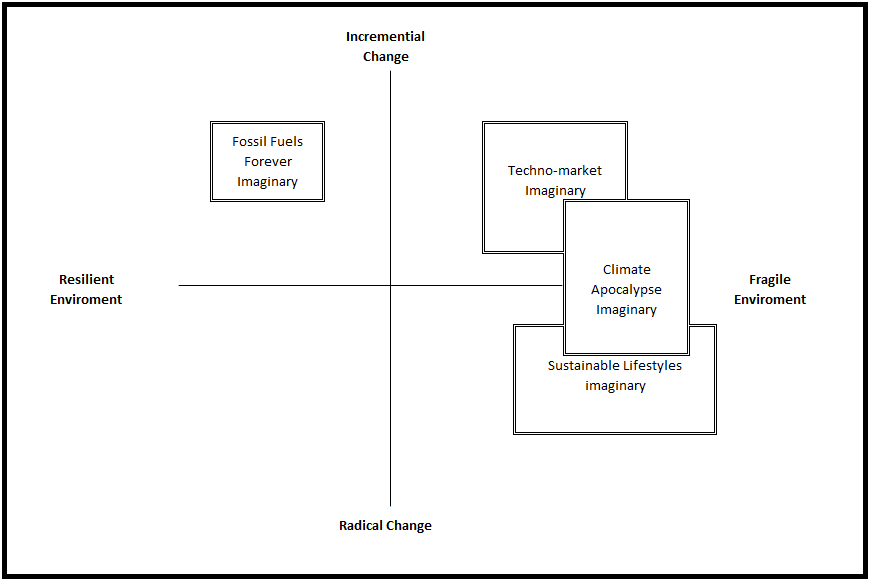
\includegraphics[width=0.75\linewidth]{C:/Users/602956/Desktop/Studie/Thesis/Sociology thesis/fig/imag_sus} 

}

\caption{ Climate Change Imaginaries (Levy and Spices, 2013) }\label{fig:clim}
\end{figure}

\subsection{Diffusion of
ECO-innovation}\label{diffusion-of-eco-innovation}

\begin{table}[t]

\caption{\label{tab:diff}Roger's five perceived components of innovations (Rogers, 1983).}
\centering
\fontsize{9}{11}\selectfont
\begin{tabular}{>{}l>{\raggedright\arraybackslash}p{30em}}
\toprule
Attributes & Definition\\
\midrule
Relative advantage & The degree to which an innovation is perceived as better than existing (economic,  advantage, social prestige, convenience, or satisfaction).\\
Compatibility & The degree to which an innovation is perceived as being consistent with the existing values, past experiences, and the needs of potential adopters.\\
Complexity & The perceived difficulty to understand and use the innovation.\\
Trialability & The degree to which the adoption of an innovation is experimented without making long-term commitments or incurring significant costs.\\
Observability & The degree to which the results of an innovation are visible to others\\
\bottomrule
\end{tabular}
\end{table}

According to Rogers (1983), the adoption of the innovations depends on
the perceived relative advantage of innovation, the complexity of the
innovation, the social influence, and required knowledge and costs. In
this article, the spread of new technology in society is conceptualized
by the process of diffusion of innovation, \enquote{the process by which
an innovation is communicated through certain channels over time among
the members of a social system.} (Rogers, 1983, p. 5). In this study,
the focus is on ECO-innovations: new products and processes which
provide customer and business value but significantly decrease
environmental impacts (James, 1997). This combination of reducing carbon
emission and provide economic opportunity's, which is also the way the
energy transition is described in the klimaatakkoord (EZK, 2019).
Innovation is communicated from individual to another via channels, that
can be things like media or personal relations. The strength of the ties
an individual maintains with a communicator of an innovation influence
the change of successful adoption. Time is involved in the speeds that
communication \enquote{passes from first knowledge of an innovation to
forming an attitude toward the innovation, to a decision to adopt or
reject, to the implementation of the new idea, and to confirm this
decision towards the rest of the world} (Rogers, 1983, p. 36). Thereby
the time that it takes to spread innovation in a social system is key in
this research. The innovation is distributed in a social system. There
are differed types of social networks, and this article focused on
private residential spatial networks. Rogers (1983) classified the
categories of the adopters as innovators, early adopters, early
majority, late majority and laggards, and innovation is spread through a
network in the respective order. This diffusion of innovation theory
leads us to conclude that the diffusion of ECO-innovation follows a
visible spatial path from innovators to the majority in a local network
trough, in which the strength of the relations influences the speed of
adoption. From this innovation theory, this article uses five steps in
the adoption process of innovation: 1) knowledge about the system and
the climate problem, 2) persuasion factors via the communication
channels, 3) way of decision making, 4) implementation, and 5)
confirmation.

\subsection{(Undetected) Social
influence}\label{undetected-social-influence}

Individuals in society do not act as independent decision-making units,
but their behavior is influenced by the other members of the reference
group (Salazar, Oerlemans, \& Stroe-Biezen, 2012), defining social
influence as the change in an individual's attitude or behavior that
results from the interaction" with other individuals or social group.
Salazar et al. (2012) studies the social influence that peer groups like
colleagues, family, and friends may have on sustainable consumption.
They find evidence for \enquote{herd behavior} (imitations of others)
and for \enquote{social learning} (learning via network). Nolan,
Schultz, Cialdini, Goldstein, and Griskevicius (2008) also investigated
the persuasive impact of normative social influence. Additionally
studied the detectability of this social influence. In the study, even
though participants expressed that social norms dod not influenced their
energy conservation, the results show a high correlation between the
descriptive norms of the network and those of the participants self. The
false perception that people have of social influence leaves the
researchers to conclude that \enquote{naive psychology-based} beliefs
about energy conservation were inaccurate predictors of actual energy
conservation. Social influence gives problems in predicting the
diffusion of ECO-innovations since peoples motivation for adoption is
less rational than they believe themselves. In this article, the focus
is on the normative frameworks on an emergent level. The aim is to
investigate how the individual believes fit in the social context of the
individual. From these emergent patterns we try to gain knowledge about
why people are not adopting ECO innovations.

\section{\texorpdfstring{Study 1: identify non-adapters
\label{Study1}}{Study 1: identify non-adapters }}\label{study-1-identify-non-adapters}

The first part of this study is about the identification (and
localization) of people that are not adopting ECO-innovation. This part
of the study is conducted as a preparation for the
\hyperref[Study2]{second part} of this article.

\subsection{Method}\label{method}

\subsubsection{Data}\label{data}

(``Stedin peer database,'' 2019) provided the data for the geographic
location of PV. This dataset contains 100.000+ locations with PV.
(``Basisregistratie adressen en gebouwen (bag),'' 2019) is used for
information about the houses in the area. (``Rotterdam in cijfers,''
n.d.) contains data about the city Rotterdam and used as a source for
the following data: residential mobility, election results, annual
income. The data about Rotterdam limits the scope of (some parts of)
this study to the Rotterdam area\footnote{I'm not sure of the whole
  scope of the project is about Rottedam, or anly for the parts where we
  do not have all the data. Specific data about residential mobility is
  only availeble for Rotterdam}.

\subsubsection{Thresholds}\label{thresholds}

Because this study views natural resources as enablers for innovation
(not as motivators), the household income is in this study used as an
interval variable. To transform the interval variable to interval
variable, this article uses the Dutch tax scales (belastingschalen)
(Belastingdienst, 2019).

\subsubsection{Procedure}\label{procedure}

Insight in the variables predicting (non-)adoption is obtained via a
multivariable regression analysis. The data is divided in separate
groups: 1) \enquote{Natural variables}, containing the natural part of
the Co-production as described by Jasanoff (2004)\footnote{Not sure is I
  can already investigate the imaginative part of Co-production in this
  part of the study. It would be nice if I could find data on a
  normative/imaginary part of this study, so I can identify social
  groups in a better way, but I cannot think of any data . Only maybe
  the data about results from voting. By doing k-fold cross validation
  it's possible to learn from the data itself if there are political
  parties that correlate with a high PV-adoption. Than it would be able
  to predict, controlled for the other variables, the adoption rate per
  party.}, and \enquote{contextual} parameters such as household income.

\subsection{Results and Discussion}\label{results-and-discussion}

\begin{table}[t]

\caption{\label{tab:RegTab}parameters regression analysis}
\centering
\fontsize{9}{11}\selectfont
\begin{tabular}{lll}
\toprule
Variable & Rotterdam & Netherlands\\
\midrule
\addlinespace[0.3em]
\multicolumn{3}{l}{\textbf{Natural resources}}\\
\hspace{1em}InstalledPV & x & x\\
\hspace{1em}HousePrice & x & x\\
\hspace{1em}SizeHouse & x & x\\
\hspace{1em}ConstructYear & x & x\\
\hspace{1em}SizeRooftop & x & x\\
\addlinespace[0.3em]
\multicolumn{3}{l}{\textbf{Contextual parameters }}\\
\hspace{1em}ResidentMobility & x & \\
\hspace{1em}Ownership & x & x\\
\hspace{1em}DistrHeat & x & x\\
\hspace{1em}Income & x & x\\
\hspace{1em}ElectionResults & x & x\\
\bottomrule
\end{tabular}
\end{table}

\section{\texorpdfstring{Study 2: Understanding non-adaptors
\label{Study2}}{Study 2: Understanding non-adaptors }}\label{study-2-understanding-non-adaptors}

Although Rogers (1983) defines lagers of innovation typically as low
educated and reluctant to change, he also argues that this group can
have real reasons for not adopting. This part of the article
investigates the arguments this from the lagers identified (and
localized) in \hyperref[Study1]{part 1} of this study by interviewing
people from this group. In this part of the study, people that are
identified as having the resources to adopt ECO-innovation, but are
however not adopting the innovation, are selected for interviewing
participants about their views on the future energy system and the role
of ECO-innovation in that view. These interviews are analyses to find
emerged patterns in the normative frameworks from this group.

\subsection{Method}\label{method-1}

\subsubsection{Participants}\label{participants}

\emph{Description of the participants based on the knowledge from part
one of this article. Dit kan nog niet helemaal worden geschreven omdat
deel 1 eerst geaadn moet worden.}

\subsubsection{Procedure}\label{procedure-1}

From the social groups that are identified as not adopting
ECO-innovation, qualitative research will be conducted in the form of
semi-structured interviews. Selecting participants consist of two parts.
The first part of the selecting process is selecting the locations for
sampling. This part is done by purposeful sampling {[}add source{]},
where we sought areas with specific characteristics that are defined in
the first part of this study. By doing so, we hoped to find
representative participants to investigate differed variables like
income, social influence and ownership of a house. The second part is
selecting the participants within the selected area. In this part the
participants were selected via a non-probability convenience sampling
(Creswell \& Poth, 2018). This procedure is chosen because it is the
(relative) most easy way to enter the field and we did not see any
reason to further complicate the selection process. Researchers went to
the selected area, \enquote{randomly}\footnote{Not sure how to write
  this} selected houses to ring doorbells and asked people for
participation.

The interviews were semi-structured. The interviews had two main focus
points: the participants view on their attributes towards ECO-innovation
(Rogers, 1983), and how they perceive the future of the climate. By
asking about how they view the relative advantage of the technique, the
compatibility with the system that they have at the moment, how they
view the complexity of the systems and it they know other people who
have the technology (Rogers, 1983). To investigate the views in the
future climate, the interview focused on the way the participants view
the stability of the eco-system and how the view change on a global
scale (Levy \& Spicer, 2013).

\subsection{Results and Discussion}\label{results-and-discussion-1}

\section{General discossion}\label{general-discossion}

\newpage

\section{References}\label{references}

\begingroup
\setlength{\parindent}{-0.5in} \setlength{\leftskip}{0.5in}

\hypertarget{refs}{}
\hypertarget{ref-BAG}{}
Basisregistratie adressen en gebouwen (bag). (2019, January).
\emph{Basisregistratie Adressen en Gebouwen (BAG)}. online database.
Retrieved from \url{https://bag.basisregistraties.overheid.nl/}

\hypertarget{ref-belastingdienst_2019}{}
Belastingdienst. (2019, January). Belastingdiens, niet aow-geregtigd.
\emph{Belastingdienst Nederland}. online database. Retrieved from
\url{https://www.belastingdienst.nl/wps/wcm/connect/bldcontentnl/belastingdienst/prive/inkomstenbelasting/heffingskortingen_boxen_tarieven/boxen_en_tarieven/overzicht_tarieven_en_schijven/u-hebt-in-2019-nog-niet-aow-leeftijd}

\hypertarget{ref-Bernards_2018}{}
Bernards, R., Morren, Johan, \& Slootweg, H. (2018). Development and
implementation of statistical models for estimating diversified adoption
of energy transition technologies. \emph{Transactions on Sustainable
Energy.}, \emph{9}(4).
doi:\href{https://doi.org/10.1109/TSTE.2018.2794579}{10.1109/TSTE.2018.2794579}

\hypertarget{ref-bogers_2010}{}
Bogers, M., Afuah, A., \& Bastian, B. (2010). Users as innovators: A
review, critique, and future research directions. \emph{Journal of
Management}, \emph{36}(4), 857--875.
doi:\href{https://doi.org/10.1177/0149206309353944}{10.1177/0149206309353944}

\hypertarget{ref-Cook_2018}{}
Cook, J. (2018). \emph{Imagined futures: Hopem risk and uncertainty}
(PhD thesis No. 7). \emph{Critical studies in risk and uncertainty}.
University of Melborne.

\hypertarget{ref-creswell_poth_2018}{}
Creswell, J. W., \& Poth, C. N. (2018). \emph{Qualitative inquiry \&
research design: Choosing among five approaches}. SAGE.

\hypertarget{ref-klimaat_2019}{}
EZK. (2019, January). Klimaatakkoord. \emph{Klimaatakkoord}. Ministerie
van Economische Zaken en Klimaat. Retrieved from
\url{https://www.klimaatakkoord.nl/}

\hypertarget{ref-gladwell_2013}{}
Gladwell, M. (2013). \emph{Outliers: The story of success}. Back Bay
Books, Little, Brown; Company.

\hypertarget{ref-ipcc_2014}{}
IPCC. (2014). AR5 synthesis report: Climate change 2014. \emph{IPCC}.
Retrieved from \url{https://www.ipcc.ch/report/ar5/syr/}

\hypertarget{ref-James_1997}{}
James, P. (1997). The sustainability circle: A new tool for product
development and design. \emph{Journal of Sustainable Product Design},
\emph{2}(52).

\hypertarget{ref-jasanoff_2004}{}
Jasanoff, S. (2004). States of knowledge: The co-production of science
and social order.
doi:\href{https://doi.org/10.4324/9780203413845}{10.4324/9780203413845}

\hypertarget{ref-Jasanoff_kim_2009}{}
Jasanoff, S., \& Kim, S.-H. (2009). Containing the atom: Sociotechnical
imaginaries and nuclear power in the united states and south korea.
\emph{Minerva}, (47), 119--146.
doi:\href{https://doi.org/\%20DOI\%2010.1007/s11024-009-9124-4}{ DOI 10.1007/s11024-009-9124-4}

\hypertarget{ref-jasanoff_kim_2015}{}
Jasanoff, S., \& Kim, S.-H. (2015). Dreamscapes of modernity :
Sociotechnical imaginaries and the fabrication of power. \emph{Chicago:
University of Chicago Press}.
doi:\href{https://doi.org/10.7208/chicago/9780226276663.001.0001}{10.7208/chicago/9780226276663.001.0001}

\hypertarget{ref-Jhagroe_2016}{}
Jhagroe, S. (2016). \emph{Urban transition politics:How struggles for
sustainability are (re)making urban spaces} (PhD thesis). Erasmus
university Rotterdam.

\hypertarget{ref-jhagroe_2015}{}
Jhagroe, S., \& Loorbach, D. (2015). See no evil, hear no evil: The
democratic potential of transition management. \emph{Environmental
Innovation and Societal Transitions}, \emph{15}, 65--83.
doi:\href{https://doi.org/10.1016/j.eist.2014.07.001}{10.1016/j.eist.2014.07.001}

\hypertarget{ref-levy_spicer_2013}{}
Levy, D. L., \& Spicer, A. (2013). Contested imaginaries and the
cultural political economy of climate change. \emph{Organization},
\emph{20}(5), 659--678.
doi:\href{https://doi.org/10.1177/1350508413489816}{10.1177/1350508413489816}

\hypertarget{ref-Buisding}{}
Lovelock, J., \& Rapley, C. (2007). Ocean pipes could help the earth to
cure itself. \emph{Nature Publishing Group}, \emph{26}(09).
doi:\href{https://doi.org/10.1093/sf/74.2.379}{10.1093/sf/74.2.379}

\hypertarget{ref-merton_1968}{}
Merton, R. (1968). The matthew effect in science. \emph{Science},
\emph{79}(159), 53--63.
doi:\href{https://doi.org/doi:10.1126/science.159.3810.56}{doi:10.1126/science.159.3810.56}

\hypertarget{ref-merton_1995}{}
Merton, R. (1995). The thomas theorem and the matthew effect.
\emph{Social Forces}, \emph{74}(2), 379--422.
doi:\href{https://doi.org/10.1093/sf/74.2.379}{10.1093/sf/74.2.379}

\hypertarget{ref-schultz_2008}{}
Nolan, J. M., Schultz, P. W., Cialdini, R. B., Goldstein, N. J., \&
Griskevicius, V. (2008). Normative social influence is underdetected.
\emph{Personality and Social Psychology Bulletin}, \emph{34}(7),
913--923.
doi:\href{https://doi.org/10.1177/0146167208316691}{10.1177/0146167208316691}

\hypertarget{ref-rogers_1983}{}
Rogers, E. M. (1983). \emph{Diffusion of innovations, 3th edition}. Free
Press.

\hypertarget{ref-rotterdam_in_cijfers}{}
Rotterdam in cijfers. (n.d.). \emph{Rotterdam in Cijfers}. Retrieved
from \url{https://rotterdam.incijfers.nl/}

\hypertarget{ref-salazar_2012}{}
Salazar, H. A., Oerlemans, L., \& Stroe-Biezen, S. V. (2012). Social
influence on sustainable consumption: Evidence from a behavioural
experiment. \emph{International Journal of Consumer Studies},
\emph{37}(2), 172--180.
doi:\href{https://doi.org/10.1111/j.1470-6431.2012.01110.x}{10.1111/j.1470-6431.2012.01110.x}

\hypertarget{ref-stedin}{}
Stedin peer database. (2019, January). company database registration PV.
Retrieved from \url{http://www.stedin.net/}

\hypertarget{ref-taylor_2004}{}
Taylor, C. (2004). Modern social imaginaries. \emph{Modern Social
Imaginaries}, 23--30.

\hypertarget{ref-DAT}{}
\emph{The day after tomorrow}. (2004).

\hypertarget{ref-vasseur_kemp_2015}{}
Vasseur, V., \& Kemp, R. (2015). The adoption of pv in the netherlands:
A statistical analysis of adoption factors. \emph{Renewable and
Sustainable Energy Reviews}, \emph{41}, 483--494.
doi:\href{https://doi.org/10.1016/j.rser.2014.08.020}{10.1016/j.rser.2014.08.020}

\hypertarget{ref-Wyatt_2003}{}
Wyatt, S. .M.E. (2003). Non-users also matter: The construction of users
and non-users of the internet. In \emph{Now users matter: The
co-construction of users and technology} (pp. 67--79). Cambridge, MA:
MIT Press.

\endgroup

\clearpage

\renewcommand{\listfigurename}{Figure captions}

\listoffigures

\clearpage

\renewcommand{\listtablename}{Table captions}

\listoftables


\end{document}
